\chapter{Dandelion++ e a vida de um nó}
\label{chapter:dandelion}
\label{page:dandelion-start}

\begin{quote}
Uma transacção não entra na rede com uma certidão de origem. Pode, contudo,
chegar cedo demais, pela porta certa e diante do vizinho errado. Há
indiscrições que não precisam de quebrar uma cifra; basta-lhes olhar para o
relógio.
\end{quote}

Até aqui construímos transacções, reunimo-las em blocos e demos ao mineiro uma
prova de trabalho. Falta acompanhar o criado discreto que leva estes objectos
de casa em casa: o nó. Quando uma carteira entrega uma transacção ao seu
daemon, ela ainda não está num bloco nem na lista de blocos. Primeiro tem de
alcançar outros nós sem anunciar com demasiada clareza onde começou. Quando um
nó novo chega à rede, pelo contrário, precisa de obter anos de blocos e
validá-los antes de saber qual é o estado corrente.

São dois movimentos da mesma vida de rede, mas não o mesmo protocolo.
Dandelion++ trata da \emph{propagação inicial de transacções}. A sincronização
trata da \emph{aquisição da lista de blocos}; a poda decide que parte da
história já validada fica disponível no disco. Reunimo-los neste capítulo
porque todos dependem das ligações e da política do nó. Separá-los-emos porque
uma flor, por diligente que seja, não sincroniza uma blockchain.

Salvo indicação em contrário, toda a descrição da implementação Monero neste
capítulo foi conferida na revisão \texttt{3646f648db57}, de 14 de Agosto de
2026 \cite{monero-source-v16}. Estes comportamentos são política de rede e de
armazenamento. Não são regras de consenso.


\section{A indiscrição da inundação}
\label{sec:dandelion-flooding}

Uma maneira simples de propagar uma transacção é a inundação
(\emph{flooding}). O nó que a recebe pela primeira vez envia-a a muitos
vizinhos; cada vizinho faz o mesmo, omitindo em geral a ligação por onde ela
chegou. A cobertura cresce depressa. Se cada nó alcançar em média \(d\)
vizinhos novos, uma árvore idealizada teria aproximadamente \(d^r\) receptores
à distância \(r\). A realidade contém ciclos, ligações lentas e nós que já
conhecem a transacção, mas a virtude continua a ser a velocidade.

A velocidade também deixa pegadas. Seja \(t_v\) o instante em que um
observador vê a transacção chegar pelo nó \(v\). Uma estimativa ingénua da
origem é
\begin{align}
 \widehat v=\underset{v}{\operatorname{argmin}}
       \bigl(t_v-\widehat\delta_v\bigr),
 \label{eq:dandelion-timing-estimator}
\end{align}
onde \(\widehat\delta_v\) é a latência que o observador atribui ao caminho até
\(v\). Não é preciso acertar em todos os atrasos. Se o adversário mantiver
muitas ligações, o primeiro vizinho honesto que lhe entregar a transacção é
frequentemente um bom candidato à origem. Esta é a estimativa do
\emph{primeiro espião} estudada no artigo Dandelion++
\cite{dandelion-plus-plus}.

Num modelo de brinquedo, cada um dos \(d\) primeiros destinatários é
controlado pelo adversário com probabilidade independente \(a\). A
probabilidade de a origem contactar logo pelo menos um espião é
\begin{align}
 P(\hbox{espião na primeira ronda})=1-(1-a)^d.
 \label{eq:dandelion-flood-first-round}
\end{align}
Com \(d=12\) e \(a=0{,}1\), o valor já é aproximadamente \(0{,}718\). Os
pares da Internet não são amostras independentes e um contacto não é uma prova
de autoria; a conta mostra apenas por que aumentar o leque inicial favorece
quem observa. O carteiro que entrega doze cópias da mesma carta é expedito, mas
não é exactamente reservado.

\begin{center}
\begin{tikzpicture}[>=stealth,node distance=.9cm and 1.1cm,
 every node/.style={font=\small},
 honest/.style={circle,draw,minimum size=.72cm,fill=blue!8},
 spy/.style={circle,draw,minimum size=.72cm,fill=red!18}]
 \node[honest,fill=green!18] (o) {origem};
 \node[honest,above right=of o] (a) {};
 \node[honest,right=of o] (b) {};
 \node[spy,below right=of o] (c) {E};
 \node[honest,right=of a] (d) {};
 \node[spy,right=of b] (e) {E};
 \node[honest,right=of c] (f) {};
 \draw[->,thick] (o)--(a);
 \draw[->,thick] (o)--(b);
 \draw[->,very thick,red!65!black] (o)--(c);
 \draw[->] (a)--(d);
 \draw[->] (a)--(e);
 \draw[->] (b)--(d);
 \draw[->] (b)--(e);
 \draw[->] (b)--(f);
 \draw[->] (c)--(e);
 \draw[->] (c)--(f);
    \node[align=center,below=.72cm of c]
   {inundação: muitos primeiros contactos;\\
    o espião \(E\) pode observar directamente a origem};
\end{tikzpicture}
\end{center}

Aleatorizar pequenos atrasos antes de cada envio dificulta
\eqref{eq:dandelion-timing-estimator}, mas não muda a forma do primeiro salto.
Dandelion++ muda-a: antes de abrir o leque, a transacção percorre uma passagem
estreita.


\section{Haste primeiro, penugem depois}
\label{sec:dandelion-stem-fluff}

Dandelion++ divide a viagem em duas fases \cite{dandelion-plus-plus}:
\begin{description}
 \item[haste (\emph{stem})] cada nó envia a transacção a um só sucessor num
 subgrafo temporário de anonimato;
 \item[penugem (\emph{fluff})] um nó difusor muda o estado da transacção e a
 envia largamente; os restantes continuam essa difusão.
\end{description}

O ponto onde começa a penugem não tem de ser o ponto de origem. Um espião que
vê primeiro a difusão pública sabe que a transacção passou por algum caminho
anterior; não sabe, só por isso, qual dos seus nós a criou.

\begin{center}
\begin{tikzpicture}[>=stealth,node distance=.95cm and .88cm,
 every node/.style={font=\small},
 dn/.style={circle,draw,minimum size=.72cm,fill=blue!8},
 fluff/.style={circle,draw,minimum size=.8cm,fill=yellow!28}]
 \node[dn,fill=green!18] (o) {O};
 \node[dn,right=of o] (s1) {1};
 \node[dn,right=of s1] (s2) {2};
 \node[fluff,right=of s2] (f) {D};
 \node[dn,above right=of f] (u1) {};
 \node[dn,right=of f] (u2) {};
 \node[dn,below right=of f] (u3) {};
 \node[dn,right=of u1] (v1) {};
 \node[dn,right=of u2] (v2) {};
 \node[dn,right=of u3] (v3) {};
 \draw[->,very thick,green!45!black] (o)--(s1);
 \draw[->,very thick,green!45!black] (s1)--(s2);
 \draw[->,very thick,green!45!black] (s2)--(f);
 \draw[->] (f)--(u1);
 \draw[->] (f)--(u2);
 \draw[->] (f)--(u3);
 \draw[->] (u1)--(v1);
 \draw[->] (u1)--(v2);
 \draw[->] (u2)--(v1);
 \draw[->] (u2)--(v2);
 \draw[->] (u2)--(v3);
 \draw[->] (u3)--(v2);
 \draw[->] (u3)--(v3);
 \node[above=.18cm of s1] {haste};
 \node[above=.18cm of u2] {penugem};
 \node[below=.18cm of o] {origem};
 \node[below=.18cm of f] {difusor};
\end{tikzpicture}
\end{center}

Suponhamos que, em cada nó de retransmissão, a probabilidade de ser difusor é
\(q\), independentemente dos anteriores. A origem faz sempre pelo menos um
salto de haste. Se \(K\) contar os saltos de haste até à transição, então
\begin{align}
 P(K=k)&=(1-q)^{k-1}q, & k&=1,2,\ldots,
 \label{eq:dandelion-geometric}\\
 P(K>k)&=(1-q)^k, & \mathbb E[K]&=\frac1q.\nonumber
\end{align}
Na implementação consultada, \(q=0{,}20\), pelo que
\(\mathbb E[K]=5\). Isto não fixa uma distância de cinco nós para cada
transacção; uma variável geométrica não faz promessas individuais. Cerca de
\(32{,}8\%\) das hastes sobrevivem a cinco decisões de retransmissão, pois
\(0{,}8^5\approx0{,}328\).

O estado essencial cabe numa transição curta:
\begin{align}
 \mathsf S
 &\xrightarrow[\text{um sucessor}]{1-q}\mathsf S,
 &
 \mathsf S
 &\xrightarrow[\text{muitos pares}]{q}\mathsf F,
 &
 \mathsf F
 &\xrightarrow[\text{muitos pares}]{}\mathsf F.
 \label{eq:dandelion-state-transition}
\end{align}
Há ainda uma seta de segurança, que não altera a ideia mas evita que um nó
malicioso guarde a carta para sempre:
\begin{align}
 \mathsf S\xrightarrow[\text{expirou o embargo}]{\text{falha segura}}
 \mathsf F.
 \label{eq:dandelion-failsafe-transition}
\end{align}


\section{O grafo que dura uma época}
\label{sec:dandelion-stem-graph}

O artigo não encaminha a haste no grafo inteiro de ligações. Em cada época,
cada nó escolhe uniformemente, sem reposição, até duas das ligações que ele
próprio iniciou. A união destas escolhas forma o subgrafo de anonimato
\(G_{\rm s}=(V,E_{\rm s})\). Cada nó tem grau de saída no máximo dois. Se as
escolhas forem aproximadamente uniformes, o grau de entrada médio também é
dois; daí a expressão «aproximadamente 4-regular». Não se exige que cada nó
receba exactamente duas arestas, nem que o grafo seja uma grinalda perfeita.

Para impedir que várias transacções vindas da mesma direcção revelem caminhos
independentes por intersecção, o artigo fixa, durante a época, uma aplicação
\begin{align}
 f_e:\ E^{\rm in}_{\rm s}(v)\longrightarrow E^{\rm out}_{\rm s}(v).
 \label{eq:dandelion-in-out-map}
\end{align}
Todas as hastes que chegam pela mesma aresta seguem pela mesma saída. A
transacção criada no próprio nó recebe igualmente uma saída persistente. No
artigo, as imagens de \(f_e\) são escolhidas pseudo-aleatoriamente com
reposição; cada nó é, durante toda a época, retransmissor ou difusor para todas
as transacções alheias. As épocas avançam assincronamente, da ordem de dez
minutos, para que a rede não troque de mapa ao toque de um sino universal
\cite{dandelion-plus-plus}.

Monero conserva a estrutura, mas não copia cada detalhe. Na revisão
consultada:
\begin{itemize}
 \item há duas hastes de saída por época, escolhidas aleatoriamente apenas
 entre ligações de saída cujo par não esteja mais de dois blocos atrasado em
 relação à altura de referência do nó;
 \item cada ligação de entrada é associada de modo persistente à haste menos
 usada; os empates são aleatórios. A origem local é representada por uma
 entrada própria e recebe a mesma espécie de associação;
 \item a época dura
 \begin{align}
  T_{\rm ep}=600\ {\rm s}+U[0,30\ {\rm s}],
  \label{eq:dandelion-monero-epoch}
 \end{align}
 após o que se renovam hastes, associações e o papel de difusor;
 \item se uma haste se desligar, o mapa tenta substituí-la por uma ligação
 elegível sem esperar pela época seguinte.
\end{itemize}
\marginnote{\scriptsize\path{src/net/dandelionpp.cpp};
\path{src/cryptonote_protocol/levin_notify.cpp}}

A escolha «menos usada» aproxima as duas cargas; não é a amostragem com
reposição do artigo. E a elegibilidade pela altura é uma necessidade do nó
Monero, não uma propriedade matemática de Dandelion++. Ser anónimo através de
um par que ainda vive anteontem seria uma vitória um tanto académica.


\section{O comportamento implementado na rede pública}
\label{sec:dandelion-monero-public}

Um nó sincronizado que recebe uma nova transacção valida-a antes de a
retransmitir. Enquanto ainda sincroniza, ignora estas notificações: não tem
estado suficiente para as tratar com utilidade. Na rede pública, uma
notificação sem a marca de penugem entra como haste; uma marcada como penugem
entra como difusão. Estes são estados da txpool e da propagação, não campos da
transacção que um mineiro compromete num bloco \cite{monero-source-v16}.

No começo de cada época, o nó torna-se difusor com probabilidade \(0{,}20\),
ou retransmissor com probabilidade \(0{,}80\). Uma transacção recebida em haste
é portanto enviada a uma só haste se o nó for retransmissor e passa à penugem
se ele for difusor. Há uma excepção deliberada: uma transacção criada
localmente faz sempre o primeiro salto de haste, mesmo durante uma época em
que o nó difunde transacções alheias. Esta excepção realiza a primeira seta de
\eqref{eq:dandelion-geometric}.

O envio por haste tenta obter e usar um destino válido. Se falhar, actualiza as
ligações e tenta uma segunda vez. Se também falhar, promove a transacção a
penugem. Se a mesma transacção chegar duas vezes como haste, o ciclo é
detectado e ela é igualmente promovida. São saídas de robustez: diminuem a
probabilidade de desaparecimento, embora uma promoção prematura encurte o
caminho de anonimato.

Na penugem, o nó prepara a transacção para todas as ligações públicas salvo a
que a forneceu. Não envia tudo no mesmo instante. Cada ligação tem uma fila e
um atraso aleatório; antes do envio, os corpos são ordenados e os duplicados
removidos, para não publicar a ordem de chegada. O protocolo corrente envia o
corpo completo da transacção. A proposta aberta \#9334 substituiria, na
penugem, estes envios redundantes por anúncios de hashes e pedidos posteriores
do corpo; em Agosto de 2026 isso continua a ser uma proposta, não comportamento
activo nem mudança de consenso \cite{monero-tx-inventory-proposal}.

O operador pode pedir enchimento das mensagens de transacções públicas até ao
múltiplo seguinte de 1024 bytes. Essa opção não está activa por omissão. O
enchimento reduz a resolução de uma análise por volume; não esconde um fluxo a
um observador capaz de correlacionar horários e direcções.


\subsection{Relógios, difusão e embargo}
\label{subsec:dandelion-timers}

Os atrasos da penugem são amostras de Poisson numa grelha de um quarto de
segundo. Para uma ligação que entrou no nó, a média é cinco segundos; para uma
ligação que o nó iniciou, é metade:
\begin{align}
 \frac{D_{\rm in}}{0{,}25\ {\rm s}}&\sim\operatorname{Pois}(20),&
 \mathbb E[D_{\rm in}]&=5\ {\rm s},
 \label{eq:dandelion-diffusion-in}\\
 \frac{D_{\rm out}}{0{,}25\ {\rm s}}&\sim\operatorname{Pois}(10),&
 \mathbb E[D_{\rm out}]&=2{,}5\ {\rm s}.
 \label{eq:dandelion-diffusion-out}
\end{align}
Assim, a difusão continua rápida sem oferecer a cada observador um relógio
determinístico.

Cada nó que guardou ou encaminhou uma transacção em haste arma também o seu
próprio embargo:
\begin{align}
 \frac{T_{\rm emb}}{1\ {\rm s}}\sim\operatorname{Pois}(39),
 \qquad \mathbb E[T_{\rm emb}]=39\ {\rm s}.
 \label{eq:dandelion-embargo}
\end{align}
Se entretanto observar a transacção em penugem, sabe que ela escapou. Se o
prazo chegar primeiro, a rotina de reenvio promove-a a difusão pública. O
prazo é local e aleatório: vários nós da haste podem armar relógios e o
primeiro a ser atendido vence. A execução não é um cronómetro de laboratório;
carga do processo e agendamento podem atrasar a chamada.

O comentário que acompanha esta constante dá como motivação
\begin{align}
 \overline T=-\frac{k(k-1)\overline h}{2\log(1-\varepsilon)}.
 \label{eq:dandelion-embargo-design}
\end{align}
Convém não transformar a motivação em consenso. A substituição dos valores ali
impressos, \(k=5\), \(\varepsilon=0{,}1\) e
\(\overline h=0{,}175\) s, dá aproximadamente \(16{,}6\) s, não 39 s. O
comportamento exacto da revisão é o de \eqref{eq:dandelion-embargo}; a conta no
comentário não altera a constante compilada.

Depois de pública, uma transacção obedece ainda à política normal da txpool:
um reenvio periódico não começa antes de cinco minutos e o intervalo cresce
até ao máximo de quatro horas. Esse relógio prolongado combate perdas comuns;
não é a falha segura Dandelion++ de 39 segundos.


\section{Tor e I2P não são uma haste mais comprida}
\label{sec:dandelion-anonymity-networks}

Quando o operador configura uma rede de anonimato para transacções locais,
Monero trata-a como uma zona própria. A integração corrente suporta Tor e I2P
e encaminha por elas transacções, não a sincronização da lista de blocos. A
sincronização pode atravessar um \emph{proxy} para endereços públicos, mas os
serviços ocultos não fornecem o protocolo completo de sincronização
\cite{monero-source-v16}.

Por omissão, a zona Tor/I2P usa ruído. Escolhe dois canais de saída por épocas
de
\begin{align}
 T_{\rm ru\acute ido}=300\ {\rm s}+U[0,30\ {\rm s}]
 \label{eq:dandelion-noise-epoch}
\end{align}
e, em cada canal, envia exactamente um fragmento de 3 KiB --- real ou
fictício --- após
\begin{align}
 D_{\rm ru\acute ido}=10\ {\rm s}+U[0,5\ {\rm s}].
 \label{eq:dandelion-noise-delay}
\end{align}
Uma mensagem real pode ocupar no máximo vinte fragmentos, cerca de 60 KiB.
Como o tamanho e o compasso dos fragmentos já fornecem cobertura, o enchimento
público de 1024 bytes não intervém.

O modo de ruído tem precedência sobre Dandelion++: não há haste Dandelion++
através desses canais. Uma transacção é posta nas duas filas cobertas e sai ao
ritmo de \eqref{eq:dandelion-noise-delay}; na ausência de mensagem, sai ruído.
Isto procura esconder a ocasião do envio a um observador do acesso à Internet,
enquanto Tor ou I2P escondem a origem da ligação ao par remoto. Se o ruído for
explicitamente desactivado, a zona usa a rotina de penugem apenas para
ligações de saída. Uma transacção recebida de Tor/I2P sem marca de penugem
recebe, antes do reencaminhamento, um atraso de Poisson de média 22 segundos.

As garantias não se somam como comprimentos de chave. Tor tem correlação de
tráfego, I2P tem outro desenho e uma população diferente; um serviço oculto
malicioso continua vendo a ligação que lhe entregou a transacção. Reutilizar
canais, ligar o daemon apenas para pagar e desligá-lo logo depois, ou permitir
a um observador moldar a largura de banda cria correlações que nenhum estado
\(\mathsf S\) apaga. A integração oficial chama experimental a esta fronteira,
com razão: a modéstia aqui é uma propriedade de segurança.


\section{O que o observador aprende}
\label{sec:dandelion-adversaries}

Comecemos por um adversário honesto-curioso que controla uma fracção \(a\) dos
nós candidatos, segue o protocolo e partilha observações. Condicionada a uma
haste de \(k\) saltos, a probabilidade idealizada de nenhum desses destinos
ser adversarial é
\begin{align}
 P(\hbox{nenhum espião}\mid K=k)=(1-a)^k.
 \label{eq:dandelion-no-spy-given-k}
\end{align}
Se em cada nó honesto há probabilidade \(q\) de começar a penugem, a
probabilidade de a haste tocar num espião antes da difusão satisfaz
\begin{align*}
 r=a+(1-a)(1-q)r,
\end{align*}
e portanto
\begin{align}
 r=\frac{a}{a+q-aq}.
 \label{eq:dandelion-spy-before-fluff}
\end{align}
Para \(a=0{,}1\) e \(q=0{,}2\), dá cerca de \(0{,}357\). Tocar num espião não
é ser identificado: o espião vê o predecessor imediato, que pode ter criado ou
apenas retransmitido a transacção. A melhoria de Dandelion++ está precisamente
em aumentar esse conjunto plausível e em resistir melhor à aprendizagem do
grafo e à intersecção de vários caminhos \cite{dandelion-plus-plus}.

O modelo independente deixa de servir quando o adversário escolhe as nossas
companhias. Muitas identidades Sybil, endereços concentrados, conhecimento do
grafo ou controlo dos pares de saída aumentam a probabilidade efectiva \(a\).
Um adversário activo pode ainda:
\begin{itemize}
 \item guardar hastes num buraco negro, forçando o embargo e observando qual
 nó acaba por difundir;
 \item encaminhar ou marcar mensagens de modo diferente para aprender o
 subgrafo;
 \item comparar várias transacções da mesma origem ao longo de épocas;
 \item combinar horários P2P com informação do fornecedor de acesso, da
 carteira, de uma bolsa ou de um destinatário.
\end{itemize}

O mapa persistente por ligação reduz o ataque de intersecção dentro de uma
época, mas não torna secreto para sempre o grafo subjacente. A renovação reduz
o valor de observações antigas, não as revoga. Um observador global passivo que
veja simultaneamente as ligações de grande parte da rede pode correlacionar a
primeira haste com a penugem posterior. Dandelion++ foi desenhado contra
desanonimização de rede em grande escala sob modelos declarados; não promete
invisibilidade perante um olho omnipresente.

Há duas fronteiras práticas importantes. Primeiro, uma carteira que usa o
daemon remoto de terceiro revela a esse daemon a ligação por onde submeteu a
transacção. Dandelion++ começa depois; não pode fabricar retrospectivamente um
salto que nunca houve. Segundo, a implementação corrente só escolhe hastes de
saída. Um nó inalcançável, que apenas estabelece ligações de saída, pode enviar
uma haste a um par que não consegue reenviá-la de volta para a população de
nós inalcançáveis. A proposta aberta do Monero Research Lab \#160 procura
permitir uma vaga de haste por ligações de entrada acompanhadas de uma prova
de limite de ligações. É investigação proposta, não código activo
\cite{monero-dandelion-inbound-proposal}.


\section{Três privacidades que não devem trocar de nome}
\label{sec:dandelion-boundaries}

\begin{description}
 \item[Anonimato da origem.] Dandelion++, Tor/I2P e os seus temporizadores
 tentam dificultar a ligação entre a primeira aparição P2P de uma transacção e
 o endereço de rede do nó que a submeteu.
 \item[Privacidade da transacção.] Endereços de utilização única, compromissos
 de montante e provas de gasto escondem destinatário, montantes e origem na
 própria transacção. Foram construídos nos capítulos
 \ref{chapter:addresses}--\ref{chapter:transactions}.
 \item[Consenso.] As regras de validação decidem se uma transacção pode entrar
 num bloco e qual cadeia possui trabalho suficiente. Dandelion++ não muda os
 bytes assinados, a imagem de chave, a prova de intervalo, a dificuldade ou a
 escolha da cadeia.
\end{description}

Uma transacção perfeitamente privada na cadeia pode denunciar o endereço IP
na rede; uma origem bem escondida pode publicar por vontade própria um
pagamento reconhecível; ambas podem ser inválidas por consenso. São eixos, não
sinónimos. Também a falha de Dandelion++ não cria moeda nem torna válido um
gasto duplo: pode revelar metadados ou atrasar propagação. Inversamente, o
consenso não garante que uma transacção ainda fora de um bloco chegue depressa
aos mineiros.


\section{Poda da blockchain e sincronização de nós podados}
\label{sec:node-pruning}

Mudamos agora de objecto. Dandelion++ transporta uma transacção recente da
txpool; a sincronização transporta blocos históricos e constrói o estado que
permitirá validar transacções futuras. Ambos pertencem à vida do nó e disputam
ligações, largura de banda, memória e disco. Não partilham, porém, fases de
haste e penugem. A poda não esconde a origem de uma transacção, e Dandelion++
não decide que história guardar.

O capítulo \ref{chapter:blockchain}, na secção
\ref{subsec:transaction-id}, já separou exactamente o material podável do
indispensável e mostrou como o hash permite reconstruir o mesmo ID. Não
repetiremos aqui a lista de campos. Interessa-nos agora a política aplicada a
essa decomposição depois da validação.


\subsection{O oitavo que não é a cadeia inteira}
\label{subsec:pruning-size}

Sejam \(S_{\rm indispensable}\) os dados que todos os nós podados conservam,
\(S_{\rm old,prunable}\) a parte podável dos blocos antigos e
\(S_{\rm recent-tip}\) a parte podável da ponta recente, que também se
conserva inteira. Para um nó podado, a conta central é
\begin{align}
 S_{\rm pruned}
   &=S_{\rm indispensable}
     +\frac18 S_{\rm old,prunable}
     +S_{\rm recent-tip},
 \label{eq:pruned-database-size}\\
 S_{\rm discarded}
   &=\frac78 S_{\rm old,prunable}.
 \label{eq:pruned-database-discarded}
\end{align}

O oitavo refere-se apenas à \emph{parte antiga podável}, não ao conjunto da
blockchain. Cabeçalhos, prefixos, dados necessários ao estado, índices e a
ponta recente não são multiplicados por \(1/8\). Por isso uma base podada não
tem um oitavo do tamanho da base completa. A documentação oficial resume a
poupança como cerca de dois terços \cite{monero-pruning-doc}; a fotografia de
Junho de 2026 no repositório Monero dava aproximadamente 280 GB para a base
completa e 95 GB para a podada, isto é,
\begin{align*}
 \frac{95}{280}\approx0{,}339.
\end{align*}
É perto de um terço, como \eqref{eq:pruned-database-size} permite esperar, e
decididamente não um oitavo.


\subsection{Faixas, semente e ponta móvel}
\label{subsec:pruning-stripes}

Fora da ponta recente, a revisão consultada divide as alturas em troços de
4096 blocos e faz rodar oito faixas. Para uma altura \(h\) e altura corrente
\(H\), a função é
\begin{align}
 \sigma(h,H)=
 \begin{cases}
  0,&h+5500\geq H,\\[1mm]
  1+\left(\left\lfloor\dfrac{h}{4096}\right\rfloor\bmod8\right),
     &h+5500<H.
 \end{cases}
 \label{eq:pruning-stripe}
\end{align}
A faixa zero é uma convenção para «ponta não podada». Um nó podado recebe
aleatoriamente uma faixa \(s\in\{1,\ldots,8\}\), conserva os dados podáveis
antigos dos troços com \(\sigma(h,H)=s\) e elimina esses dados nos outros sete
troços. A escolha e o expoente \(\log_2 8=3\) são codificados na
\emph{semente de poda}. Ela identifica uma política; não é uma semente capaz
de regenerar as provas apagadas.
\marginnote{\scriptsize\path{src/common/pruning.cpp};
\path{src/cryptonote_config.h}}

\begin{center}
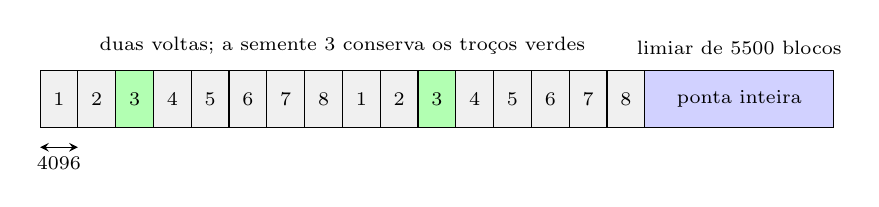
\begin{tikzpicture}[x=.48cm,y=.72cm,>=stealth,
 every node/.style={font=\scriptsize}]
 \foreach \x/\s in {0/1,1/2,2/3,3/4,4/5,5/6,6/7,7/8,
                     8/1,9/2,10/3,11/4,12/5,13/6,14/7,15/8}{
   \ifnum\s=3
     \fill[green!30] (\x,0) rectangle ++(1,1);
   \else
     \fill[gray!12] (\x,0) rectangle ++(1,1);
   \fi
   \draw (\x,0) rectangle ++(1,1);
   \node at (\x+.5,.5) {\s};
 }
 \fill[blue!18] (16,0) rectangle (21,1);
 \draw (16,0) rectangle (21,1);
 \node[align=center] at (18.5,.5) {ponta inteira};
 \draw[<->] (0,-.35)--(1,-.35) node[midway,below] {4096};
 \node[align=center,above] at (8,1.12)
   {duas voltas; a semente 3 conserva os troços verdes};
 \node[align=center,above] at (18.5,1.12) {limiar de 5500 blocos};
\end{tikzpicture}
\end{center}

À medida que \(H\) avança, a janela recente avança com ele. Em operações de
manutenção, o nó examina os dados que acabaram de sair da condição
\(h+5500\geq H\): conserva-os se pertencem à sua faixa e liberta-os se não
pertencem. A ponta inteira ajuda a servir os blocos recentes e as
reorganizações usuais; 5500 não é uma promessa de finalidade. O consenso
continua a poder escolher uma reorganização válida mais profunda.


\subsection{O que um nó podado oferece à rua}
\label{subsec:pruning-serving}

Um nó podado pode fornecer a qualquer par os blocos e as partes indispensáveis
da história, os dados podáveis completos da sua faixa e todos os dados da
ponta recente. Não pode servir uma prova histórica que apagou. Um nó completo,
representado por semente zero no protocolo, pode servir qualquer faixa.

A escolha aleatória de \(s\) encoraja cobertura distribuída. Se \(n\) nós
podados escolhessem faixas independentemente e não houvesse nós completos, a
probabilidade de uma faixa fixada não aparecer seria
\begin{align}
 \left(\frac78\right)^n,
 \label{eq:pruning-missing-one-stripe}
\end{align}
e, pela união dos oito acontecimentos, a probabilidade de faltar pelo menos
uma faixa seria no máximo
\begin{align}
 8\left(\frac78\right)^n.
 \label{eq:pruning-missing-any-stripe}
\end{align}
É um incentivo estatístico, não uma obrigação. Operadores podem copiar bases,
escolher a mesma faixa, ficar desligados ou desaparecer. As regras de consenso
validam blocos; não enviam meirinhos contar discos privados. Logo, a cobertura
de todas as faixas é desejada pela política de rede, mas não garantida pelo
consenso.


\subsection{Três percursos de sincronização}
\label{subsec:pruned-sync-modes}

É útil separar três percursos que a expressão «sincronização podada» costuma
meter no mesmo saco.

\paragraph{Validar primeiro, podar depois.}
Um nó pode sincronizar uma base completa, receber cada prova histórica,
validar blocos e transacções e só depois executar a poda local. Nesse percurso,
a decisão de apagar vem depois da verificação independente. Podar uma LMDB já
existente marca páginas como livres para reutilização e pode não encolher logo
o ficheiro; a ferramenta de cópia podada cria uma base fisicamente menor.

\paragraph{Começar do zero com poda activada.}
Com \texttt{--prune-blockchain}, o daemon cria desde o início uma semente e
mantém a base segundo \eqref{eq:pruning-stripe}. Na revisão consultada, esta
opção, por si só, não activa \texttt{--sync-pruned-blocks}. O nó pede material
completo a pares capazes de servir cada faixa, valida-o e vai libertando
localmente os sete oitavos antigos que não lhe cabem. Poupa disco durante o
crescimento, mas não deve ser descrito como se aceitasse automaticamente
provas já ausentes.

\paragraph{Aceitar história que já chegou podada.}
A opção adicional \texttt{--sync-pruned-blocks} autoriza pedidos de respostas
podadas quando a base local também tem uma semente. O pedido só é feito se
todas estas condições se verificarem na revisão de Agosto de 2026:
\begin{itemize}
 \item o intervalo não pertence à faixa local nem à ponta recente;
 \item começa pelo menos na altura ideal da versão 11, porque antes dela o nó
 não reconstrói por esta via o peso necessário;
 \item o último bloco do intervalo está dentro da zona de hashes de blocos
 compilados no programa;
 \item os pesos de todos os blocos pedidos já constam dessa informação
 compilada.
\end{itemize}
Se uma condição falhar, o nó pede dados completos. Assim se compreende a frase
documental «sincronizar só cerca de um terço»: descreve o efeito do percurso
que aceita história podada onde ele é permitido, não uma identidade universal
entre \texttt{--prune-blockchain} e uma descarga de \(1/8\).
\marginnote{\scriptsize\path{src/cryptonote_protocol/}
\path{cryptonote_protocol_handler.inl}}


\subsection{Verificar um hash não verifica uma prova ausente}
\label{subsec:pruned-sync-validation}

Numa resposta podada, o par fornece o bloco, a base de cada transacção, o hash
da parte podável e o peso necessário. O nó consegue reconstruir o ID da
transacção, confirmar que esse ID aparece no bloco, encadear cabeçalhos e
construir o estado indispensável. Recusa uma resposta podada quando tinha
pedido uma completa e recusa pesos nulos onde esperava dados podados.

O que ele não consegue fazer é recalcular uma prova criptográfica cujos bytes
não recebeu. Para os intervalos aceites por
\texttt{--sync-pruned-blocks}, a correspondência com os hashes e pesos
compilados ancora a história à fotografia distribuída com o programa. Um par
não pode trocar livremente a prova ausente por outra história sem mudar os
IDs; mas o nó também não obtém, nessa sincronização, uma reverificação
independente das assinaturas e provas removidas. Confia que a história
comprometida pelos pontos de controlo foi validada antes da sua compilação.

Esta fronteira é exacta e saudável de declarar. Uma sincronização completa
seguida de poda pode dizer: «eu verifiquei e depois apaguei». Uma sincronização
que aceitou a história podada diz: «verifiquei o que recebi e prendi-o ao
compromisso distribuído; a prova antiga já não estava presente». Ambos aplicam
normalmente as regras aos blocos novos e conservam a mesma capacidade funcional
corrente, mas o percurso de confiança histórico não é idêntico.


\subsection{Encontrar a faixa seguinte}
\label{subsec:pruned-peer-selection}

Durante a apresentação P2P, cada par anuncia a sua semente de poda. O receptor
aceita a semente zero, que significa base completa, ou uma semente com
\(\log_2 8=3\) e faixa entre 1 e 8; valores incompatíveis levam ao fecho da
ligação. A fila de blocos calcula a faixa da próxima altura necessária.

Sem \texttt{--sync-pruned-blocks}, o nó procura um par completo ou um par cuja
faixa contenha material integral para esse troço. Pode reservar desde já o
troço da faixa seguinte e liberta ligações pouco úteis para abrir lugar à
faixa necessária. Com a opção activa, qualquer par que conserve a base
indispensável pode responder de forma podada aos troços que o nó local não
pretende conservar; para a faixa local e para a ponta, continuam necessários
dados completos. A semente anunciada permite escolher sem pedir a um vizinho o
livro que ele já declarou ter queimado.

Perto do topo, \(\sigma=0\) para todos. Os pares podados conservam os dados
completos da janela e podem servi-los; a validação corrente não depende de
hashes históricos compilados. Numa reorganização normal dentro dessa janela,
o nó possui ou descarrega as transacções e provas completas da nova rama. Se
uma reorganização excepcional exigir uma rama profunda fora da janela, um nó
podado tem de encontrar pares que forneçam o material integral que falta; uma
rama alternativa nova não pode ser justificada por um hash compilado da antiga
cadeia principal. A poda não transforma 5500 blocos em finalidade e a falha de
cobertura pode atrasar ou impedir aquele nó de acompanhar a reorganização.


\section{O que a flor promete, e só isso}
\label{sec:dandelion-summary}

Dandelion++ coloca um caminho estreito e renovável antes da difusão. As duas
hastes, o mapa persistente por entrada, o papel de difusor e o embargo tornam
menos convincente a conclusão «vi primeiro, logo criou». A implementação
Monero acrescenta filtros de altura, equilíbrio das hastes, difusão com
atrasos, detecção de ciclos e uma falha segura concreta. Tor/I2P, quando
configurados, usam canais e ruído próprios; propostas para hastes de entrada e
anúncios por inventário continuam propostas.

Nada disto oculta uma carteira de um daemon remoto, derrota um observador
global, garante propagação contra todos os nós maliciosos ou altera consenso.
É uma defesa probabilística de metadados, com hipóteses e falhas observáveis.

A poda responde a outra escassez. Conserva tudo o que o nó precisa para o
estado corrente, um oitavo da parte antiga podável e a ponta recente inteira.
As oito faixas tornam provável que a rede retenha cópias, mas nenhuma regra de
consenso garante que os respectivos proprietários estejam amanhã em casa.
Sincronizar com dados completos e apagá-los depois não é o mesmo que aceitar
uma história já podada; saber qual dos dois percursos se tomou vale mais do que
chamar «sem confiança» a ambos e esperar que o adjectivo faça a verificação.

O nó, enfim, tem duas prudências. Ao falar, procura não dizer de onde veio a
transacção. Ao arrumar, procura não deitar fora tudo aquilo de que a rede ainda
pode precisar. A primeira prudência chama-se Dandelion++; a segunda, poda.
Confundi-las pouparia uma secção e perderia o capítulo.

\label{page:dandelion-end}
